\documentclass[tikz,border=2mm]{standalone}
\usepackage{tikz}
\usetikzlibrary{arrows.meta,positioning,shapes.geometric}

\begin{document}
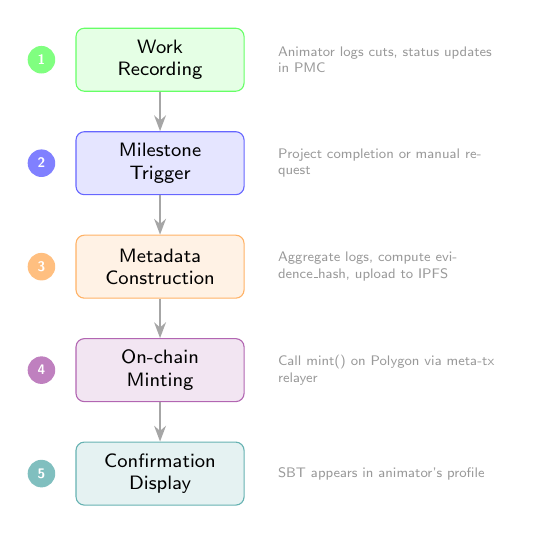
\begin{tikzpicture}[
  node distance=0.5cm and 0.2cm,
  step/.style={
    rectangle, rounded corners=3pt, draw=#1!60, fill=#1!10,
    minimum width=2.0cm, minimum height=0.8cm,
    text width=1.9cm, align=center, font=\scriptsize\sffamily
  },
  arrow/.style={-{Stealth[length=2mm]}, thick, draw=gray!70},
  lbl/.style={font=\tiny\sffamily, text=gray!80},
  num/.style={circle, fill=#1!50, text=white, font=\tiny\bfseries\sffamily,
    minimum size=3.5mm, inner sep=0pt}
]

% Steps - vertical layout
\node[step=green] (s1) {Work\\Recording};
\node[step=blue, below=of s1] (s2) {Milestone\\Trigger};
\node[step=orange, below=of s2] (s3) {Metadata\\Construction};
\node[step=violet, below=of s3] (s4) {On-chain\\Minting};
\node[step=teal, below=of s4] (s5) {Confirmation\\Display};

% Step numbers
\node[num=green, left=0.25cm of s1] {1};
\node[num=blue, left=0.25cm of s2] {2};
\node[num=orange, left=0.25cm of s3] {3};
\node[num=violet, left=0.25cm of s4] {4};
\node[num=teal, left=0.25cm of s5] {5};

% Arrows
\draw[arrow] (s1) -- (s2);
\draw[arrow] (s2) -- (s3);
\draw[arrow] (s3) -- (s4);
\draw[arrow] (s4) -- (s5);

% Right-side annotations
\node[lbl, right=0.3cm of s1, text width=2.8cm] {Animator logs cuts, status updates in PMC};
\node[lbl, right=0.3cm of s2, text width=2.8cm] {Project completion or manual request};
\node[lbl, right=0.3cm of s3, text width=2.8cm] {Aggregate logs, compute evidence\_hash, upload to IPFS};
\node[lbl, right=0.3cm of s4, text width=2.8cm] {Call mint() on Polygon via meta-tx relayer};
\node[lbl, right=0.3cm of s5, text width=2.8cm] {SBT appears in animator's profile};

\end{tikzpicture}
\end{document}
